	
\begin{frame}
\large Current Work\\

	\begin{itemize}
		\item Finding the optimal size of a reactor to minimize the cost of electricity and steam. \\
                \item The method will use RAVEN (Rabiti, INL), and will be based on a paper 
                        \cite{baker_optimal_2018} that sized a reactor for a 
                        similar grid system.
	\end{itemize}
        \begin{figure}
                \centering
                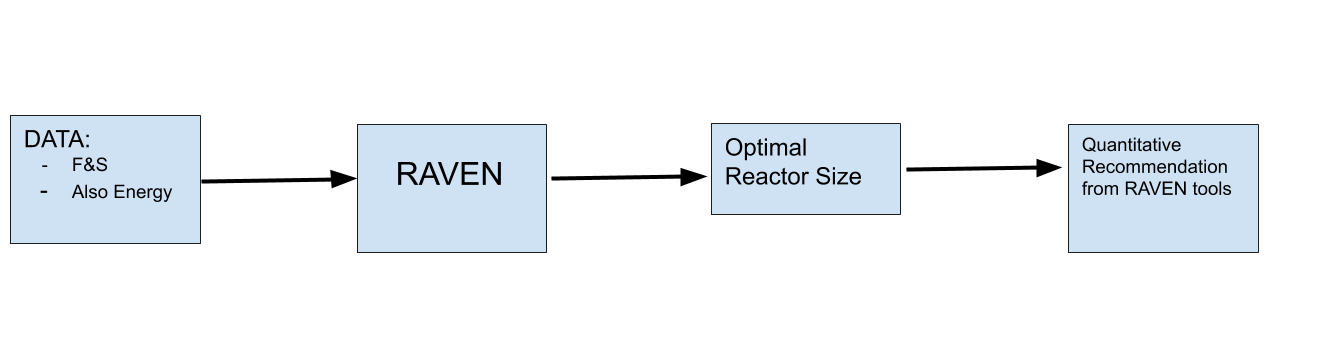
\includegraphics[height=0.5\textheight]{./images/flow.png}
                \caption{Work Plan.}
        \end{figure}
\end{frame}

\begin{frame}
        F\&S intends to retire the coal boilers by 2030 and replace them with 
        ``Developing Technologies,'' according to the Utilities Master plan 
        \cite{affiliated_engineers_inc_utilities_2015}. Without new 
        technologies available, the current plan is to replace this capacity 
        with  more PPAs and natural gas 
        \cite{affiliated_engineers_inc_utilities_2015}. However, small nuclear 
        power was mentioned as a possible ``developing technology'' which could 
        be considered if ready in time. 

	\begin{figure}
		\centering
		\label{fig:masterplan}
		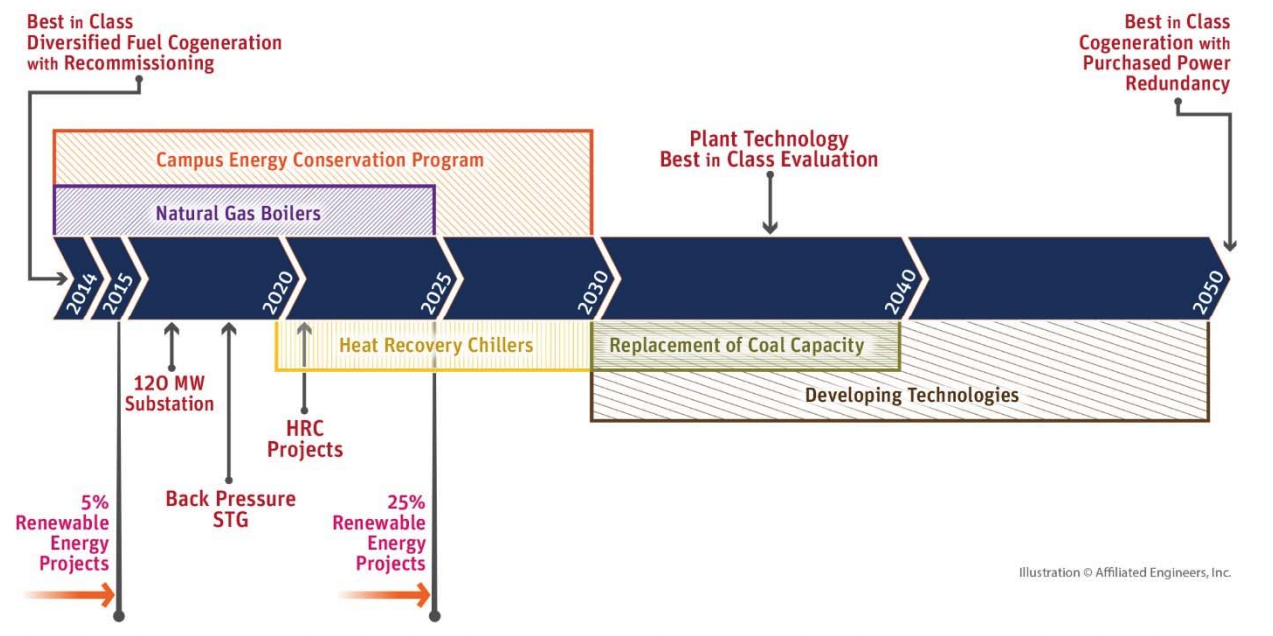
\includegraphics[width=0.75\textwidth]{./images/masterplan.png}
		\caption{Current trajectory suggests that campus should ``Re-evaluate and apply best of industry energy supply utilizing future advanced
technology and innovations for plant repowering in the 2030-2040 time frame.'' 
                \cite{affiliated_engineers_inc_utilities_2015}.}
	\end{figure}
\end{frame}
